\section{Model 2: Transfer Learning with ResNet-50}
\label{sec:model2}

\subsection{Methods}

The second backbone evaluated for Model 2 is a ResNet-50 pretrained on ImageNet
\cite{he2016resnet}. As with EfficientNet-B0, the network does not learn all
features from scratch but starts from weights that already encode general visual
features such as edges, textures, and shapes. These features can be reused for
satellite imagery classification with only minimal adaptation. Evaluating a
second, structurally different backbone makes the comparison with the scratch CNN
more robust: a consistent advantage across both ResNet-50 and EfficientNet-B0
indicates that the benefit stems from transfer learning itself rather than from a
single architecture.

ResNet-50 was chosen for this second backbone because it is a canonical, larger
deep-residual network and therefore complements the compact EfficientNet-B0: the
two cover different architecture families and capacities (roughly 25 versus 5
million parameters). It is a widely used reference for transfer learning, which
keeps the results comparable to the literature. Its clearly separated residual
stages (\texttt{layer1}--\texttt{layer4}) also make staged fine-tuning
straightforward, and high-quality ImageNet-pretrained weights
(\texttt{IMAGENET1K\_V2}) are readily available.

\subsubsection{ResNet-50 Architecture}

ResNet-50 is a deep residual network with 50 layers organized into four residual
stages, followed by a global average pooling layer and a fully connected
classification head. The defining feature of ResNet is the residual connection:
each block adds its input directly to its output before the activation. This
skip connection addresses the vanishing gradient problem and allows very deep
networks to be trained stably \cite{he2016resnet}.

\begin{table}[H]
\centering
\caption{ResNet-50 architecture overview. Feature map sizes assume 224$\times$224 input.}
\label{tab:resnet_architecture}
\begin{tabularx}{\textwidth}{lXX}
\toprule
Stage & Layers & Output size \\
\midrule
Input   & RGB image                          & 3$\times$224$\times$224 \\
Conv1   & 7$\times$7 conv, stride 2, MaxPool & 64$\times$56$\times$56  \\
Layer1  & 3 bottleneck blocks                & 256$\times$56$\times$56 \\
Layer2  & 4 bottleneck blocks                & 512$\times$28$\times$28 \\
Layer3  & 6 bottleneck blocks                & 1024$\times$14$\times$14 \\
Layer4  & 3 bottleneck blocks                & 2048$\times$7$\times$7  \\
Head    & GlobalAvgPool, Linear              & $C$ logits              \\
\bottomrule
\end{tabularx}
\end{table}

Each bottleneck block consists of three convolutional layers (1$\times$1, 3$\times$3,
1$\times$1) with batch normalization and ReLU activations. The 1$\times$1 layers
reduce and then restore the channel dimension, while the 3$\times$3 layer performs
the spatial feature extraction. This design keeps the parameter count manageable
despite the network depth.

\subsubsection{Transfer Learning Setup}

The pretrained weights were loaded from torchvision using the
\texttt{IMAGENET1K\_V2} checkpoint \cite{torchvision}. In the transfer learning
setup, the backbone is initially fully frozen and only the classification head is
replaced. The original fully connected layer, which outputs 1000 ImageNet
classes, is replaced by a new linear layer mapping the 2048-dimensional feature
vector to 10 outputs for the multiclass task or 2 outputs for the binary task.

All backbone parameters except those in the last residual stage (\texttt{layer4})
are kept frozen throughout training. The unfreezing of \texttt{layer4} allows the
network to adapt its highest-level features to the specific visual characteristics
of satellite imagery while keeping the low- and mid-level texture features fixed.
This strategy follows the standard practice of fine-tuning only the deeper layers,
since earlier layers in convolutional networks learn general low-level features
that transfer well across domains \cite{yosinski2014transferable}.

The key configuration differences from the scratch CNN are:

\begin{itemize}
  \item Input images are resized to 224$\times$224 (instead of 64$\times$64), matching the
    input resolution the backbone was pretrained on.
  \item Normalization uses ImageNet statistics: mean $[0.485, 0.456, 0.406]$ and
    standard deviation $[0.229, 0.224, 0.225]$ per channel. This ensures the
    input distribution matches what the frozen layers expect.
  \item The learning rate is set to $1\times10^{-4}$ (compared to $1\times10^{-3}$
    for the scratch CNN). A lower rate is important for fine-tuning to avoid
    overwriting the pretrained features with large gradient updates.
  \item The optimizer is Adam with weight decay $1\times10^{-4}$.
  \item Training runs for up to 50 epochs with early stopping after 8 epochs
    of no improvement in validation loss.
\end{itemize}

The number of trainable parameters with \texttt{layer4} unfrozen is 14{,}985{,}226.
For comparison, the fully frozen variant trains only the classification head,
giving 20{,}490 trainable parameters.

\subsection{Experimental Design}
\label{sec:model2_experiments}

Two sets of experiments were used to characterize the transfer learning model.

The first set tests \textbf{data efficiency}: how much labeled training data does
each model need to reach competitive accuracy? Both the ResNet and the scratch CNN
were trained on three progressively larger subsets of the training data, keeping
the full validation and test splits constant for fair comparison. Additionally, a
fully frozen ResNet was trained at full data as a baseline to isolate the
contribution of fine-tuning over using pretrained ImageNet features alone.

\begin{table}[H]
\centering
\caption{Data efficiency experiments. All runs use the multiclass task and
evaluate on the full test split ($n=4050$).}
\label{tab:data_efficiency_exp}
\begin{tabular}{llrrr}
\toprule
ID & Model & Train images & Test Acc. & Test Macro-F1 \\
\midrule
S-50    & Scratch CNN       &    500 & 0.7017 & 0.6904 \\
S-200   & Scratch CNN       &  2{,}000 & 0.8430 & 0.8379 \\
S-full  & Scratch CNN       & 18{,}899 & 0.9479 & 0.9462 \\
\midrule
R-50    & ResNet (layer4)   &    500 & 0.9284 & 0.9263 \\
R-200   & ResNet (layer4)   &  2{,}000 & 0.9556 & 0.9542 \\
R-full  & ResNet (layer4)   & 18{,}899 & 0.9817 & 0.9812 \\
\midrule
R-frz   & ResNet (frozen)   & 18{,}899 & 0.9373 & 0.9347 \\
\bottomrule
\end{tabular}
\end{table}

The second set applies the same data efficiency design to the \textbf{binary
vegetation task}.

\begin{table}[H]
\centering
\caption{Data efficiency experiments on the binary classification task.
Test split $n=4050$.}
\label{tab:data_efficiency_binary}
\begin{tabular}{llrrr}
\toprule
ID & Model & Train images & Test Acc. & Test Macro-F1 \\
\midrule
S-50-b   & Scratch CNN     &    500 & 0.8691 & 0.8691 \\
S-200-b  & Scratch CNN     &  2{,}000 & 0.9081 & 0.9081 \\
S-full-b & Scratch CNN     & 18{,}899 & 0.9741 & 0.9741 \\
\midrule
R-50-b   & ResNet (layer4) &    500 & 0.9753 & 0.9753 \\
R-200-b  & ResNet (layer4) &  2{,}000 & 0.9889 & 0.9889 \\
R-full-b & ResNet (layer4) & 18{,}899 & 0.9938 & 0.9938 \\
\bottomrule
\end{tabular}
\end{table}

\subsection{Results}

\subsubsection{Final 10-Class Classification}

The final ResNet model (R-full, \texttt{layer4} unfrozen, full training data)
achieves the results shown in Table \ref{tab:resnet_final_multiclass}. The model
converged in 15 epochs before early stopping triggered.

\begin{table}[H]
\centering
\caption{Final ResNet-50 results for the 10-class classification task.}
\label{tab:resnet_final_multiclass}
\begin{tabular}{lrr}
\toprule
Metric & Validation & Test \\
\midrule
Loss     & 0.0732 & 0.0618 \\
Accuracy & 0.9780 & 0.9817 \\
Macro-F1 & 0.9770 & 0.9812 \\
\bottomrule
\end{tabular}
\end{table}

\begin{figure}[H]
\centering
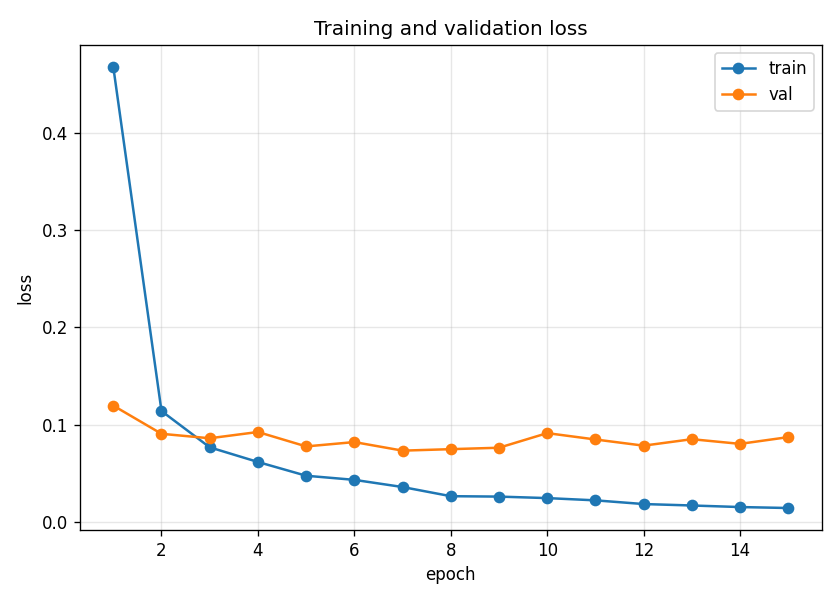
\includegraphics[width=0.78\textwidth]{../outputs/experiments/scratch_vs_transfer/runs/resnet_full/plots/loss_curve.png}
\caption{Loss curve of the final ResNet-50 10-class model.}
\label{fig:resnet_loss}
\end{figure}

\begin{figure}[H]
\centering
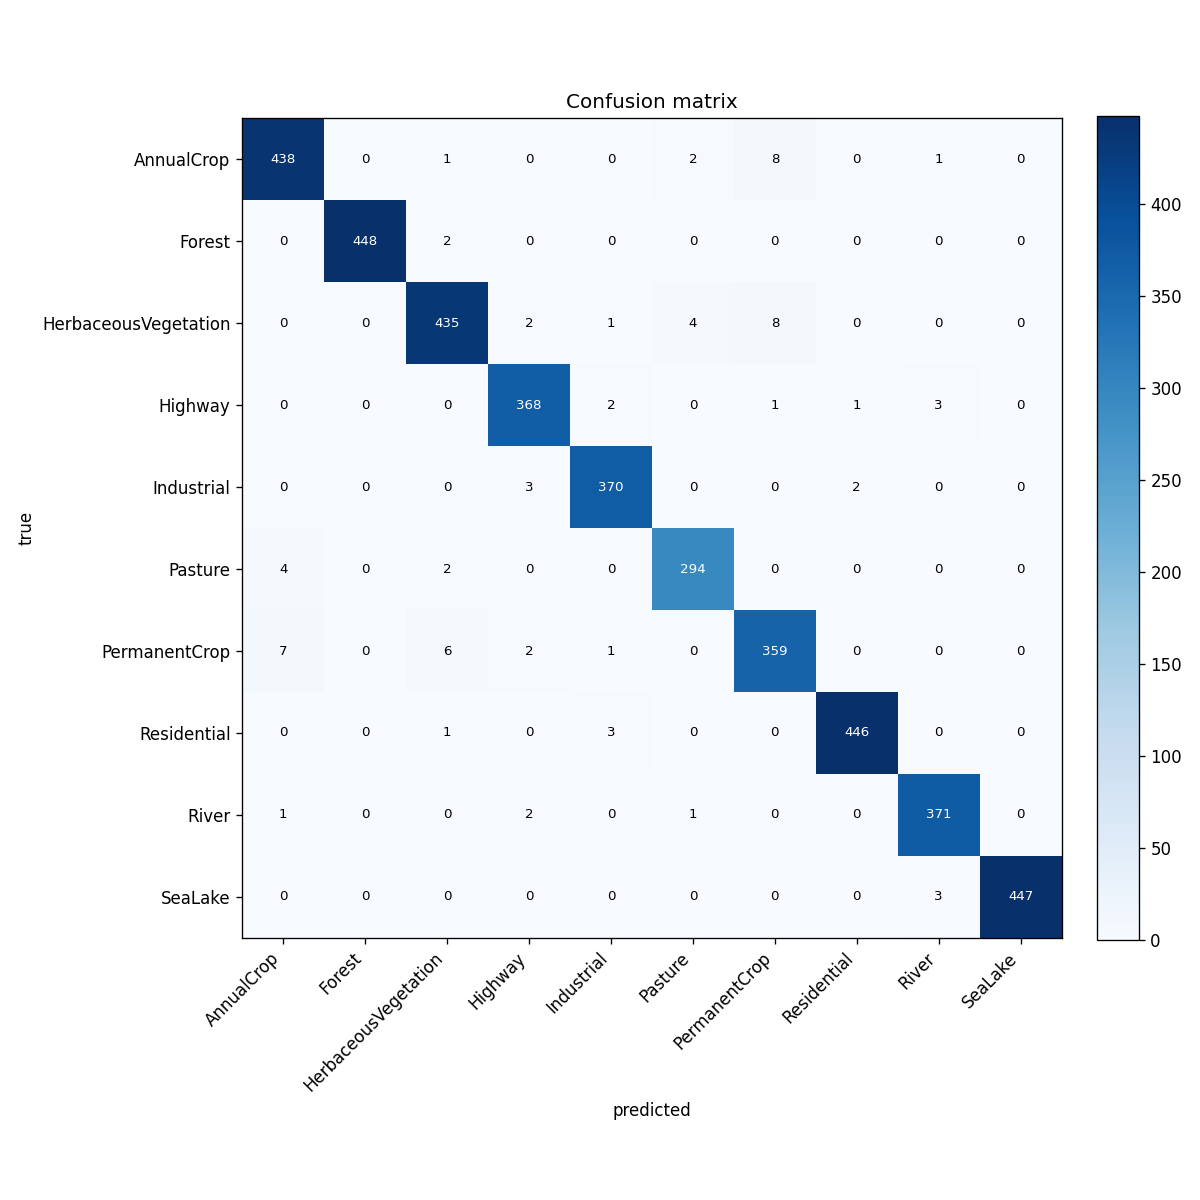
\includegraphics[width=0.78\textwidth]{../outputs/experiments/scratch_vs_transfer/runs/resnet_full/plots/confusion_matrix.png}
\caption{Confusion matrix of the final ResNet-50 10-class model on the test split.}
\label{fig:resnet_cm}
\end{figure}

\begin{table}[H]
\centering
\caption{Per-class test results of the final ResNet-50 10-class model.}
\label{tab:resnet_per_class}
\small
\begin{tabular}{lrrrr}
\toprule
Class & Precision & Recall & F1 & Support \\
\midrule
AnnualCrop            & 0.9733 & 0.9733 & 0.9733 & 450 \\
Forest                & 1.0000 & 0.9956 & 0.9978 & 450 \\
HerbaceousVegetation  & 0.9732 & 0.9667 & 0.9699 & 450 \\
Highway               & 0.9761 & 0.9813 & 0.9787 & 375 \\
Industrial            & 0.9814 & 0.9867 & 0.9840 & 375 \\
Pasture               & 0.9767 & 0.9800 & 0.9784 & 300 \\
PermanentCrop         & 0.9548 & 0.9573 & 0.9561 & 375 \\
Residential           & 0.9933 & 0.9911 & 0.9922 & 450 \\
River                 & 0.9815 & 0.9893 & 0.9854 & 375 \\
SeaLake               & 1.0000 & 0.9933 & 0.9967 & 450 \\
\bottomrule
\end{tabular}
\end{table}

On the test split, 3976 out of 4050 images were classified correctly, leaving
74 misclassifications. The weakest class is PermanentCrop (F1 0.9561), which is
also the hardest class for the scratch CNN. The strongest classes are Forest and
SeaLake, both achieving near-perfect precision. The overall per-class scores are
notably more uniform than for the scratch CNN, suggesting that the pretrained
features generalize better across visually similar classes.

\subsubsection{Final Binary Classification}

The binary ResNet model (R-full-b) achieves the results shown in Table
\ref{tab:resnet_final_binary}. The model converged in 12 epochs.

\begin{table}[H]
\centering
\caption{Final ResNet-50 results for the binary classification task.}
\label{tab:resnet_final_binary}
\begin{tabular}{lrr}
\toprule
Metric & Validation & Test \\
\midrule
Loss     & 0.0165 & --- \\
Accuracy & 0.9943 & 0.9938 \\
Macro-F1 & 0.9943 & 0.9938 \\
\bottomrule
\end{tabular}
\end{table}

\begin{figure}[H]
\centering
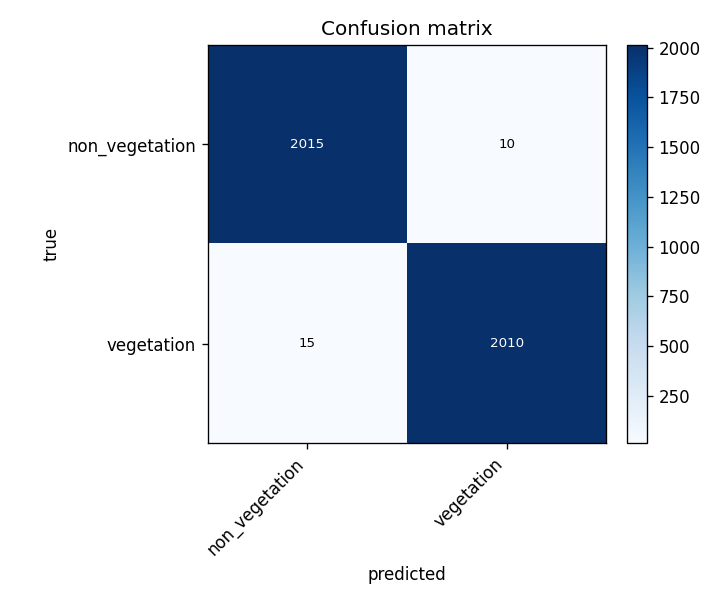
\includegraphics[width=0.7\textwidth]{../outputs/experiments/scratch_vs_transfer/runs/resnet_full_binary/plots/confusion_matrix.png}
\caption{Confusion matrix of the final ResNet-50 binary model on the test split.}
\label{fig:resnet_binary_cm}
\end{figure}

On the binary task the model misclassifies only 25 out of 4050 images. Both
vegetation and non-vegetation classes are handled with nearly equal accuracy,
indicating that the pretrained features already capture the spectral and textural
distinction between these two categories very reliably.
